\chapter{Implementacija i korisničko sučelje}
		
		
		\section{Korištene tehnologije i alati}
			
			\textit{}Za svakodnevnu komunikaciju korištena je aplikacija \underline{WhatsApp}\footnote[1]{https://www.whatsapp.com/} dok smo za sastanke i videopozive koristili platformu \underline{MS Teams}\footnote[2]{https://www.microsoft.com/en-ww/microsoft-365/microsoft-teams/group-chat-software}. Za izradu UML dijagrama i svih tablica korištena je web aplikacija \underline{Creatly}\footnote[3]{https://www.creately.com/}. Dokumentacija je pisana pomoću online Latex editora \underline{Overleaf}\footnote[4]{https://www.overleaf.com/}. Kao sustav za upravljanje izvornim kodom korišten je \underline{Git}\footnote[5]{https://git-scm.com/} dok se udaljeni repozitorij projekta nalazi na web platformi \underline{GitLab}\footnote[6]{https://gitlab.com/}.
			
			\textit{}Kao razvojno okruženje za backend je korišten \underline{IntelliJ}\footnote[7]{https://www.jetbrains.com/idea/} - integrirano razvojno okruženje (IDE) napisano u Javi za razvoj računalnog softvera. Razvio ga je JetBrains (prije poznat kao IntelliJ) i dostupan je pod licencom Apache 2. Može se koristit na svim operacijskim sustavima, koristi se za razvoj web-stranica i web-aplikacija. Frontend je napisan u \underline{Visual Studio Code}\footnote[8]{https://code.visualstudio.com/} - source-code editor koji je razvijen od tvrtke Microsoft. Zaštićen je pod MIT licencom. VSC podržava programiranje u raznim jezicima kao što su Java, JavaScript, Go, Node.js and C++. Velika prednost je što se mogu instalirati proširenja koja mogu pružiti podršku za nove jezike, teme ili debuggere. Također podržava rad sa JSON, CSS i HTML tipovima podataka što omogućuje razvoj web-stranica i web-aplikacija.
			
			\textit{}Aplikacija je napisana koristeći radni okvir \underline{Spring Framework}\footnote[9]{https://spring.io/} i jezik \underline{Java}\footnote[10]{https://www.java.com/en/} za izradu backenda dok je za frontend korišten \underline{React}\footnote[11]{https://reactjs.org/} i jezik \underline{JavaScript}\footnote[12]{https://developer.mozilla.org/en-US/docs/Web/JavaScript}. Spring Framework je otvorenog koda i sadrži gotove funkcionalnosti koji se mogu koristiti u svakoj Java aplikaciji, ali postoje i proširenja za izradu same aplikacije. React je JavaScript biblioteka koja se koristi za razvoj korisničkih sučelja i UI komponenti. Održavan je  od strane Facebooka i zajednice programera i kompanija. Može se koristiti kao baza za jednostavne stranice ili aplikacije, ali za složeniju upotrebu je potrebno koristiti dodatne biblioteke kao što su Redux i React Router, jer se React zapravo samo bavi prikazom podataka u DOM-u (Document Object Model).
			
			\textit{}Baza podataka nalazi se na poslužitelju u oblaku \underline{Heroku}\footnote[13]{https://www.heroku.com/}, a za relacijsku bazu 
			podataka korišten je \underline{PostgreSQL}\footnote[14]{https://www.postgresql.org/}.
			
			\eject 
		
	
		\section{Ispitivanje programskog rješenja}	
			
			\subsection{Ispitivanje komponenti}
			
			Za ispitivanje razrednih funkcija koje implementiraju temeljne funkcionalnosti koristili smo MockMvc. MockMvc je razred definiran u javi pomoću kojeg možemo kontrolerima poslati lažne HTTP zahtjeve i testirati njihovo  ponašanje bez pokretanja kontrolera unutar poslužitelja.U nastavku će biti prikazani neke od metoda koje smo testirali i odlučili prikazati.
			
			 \noindent \underbar{\textbf{1. Dohvati sve teretane}}
			 
             Ovdje smo testirali pokušaj dohvaćanja teretana odlaskom na /getGyms.

			\begin{figure}[H]
    			\hspace*{-1.5cm}
    			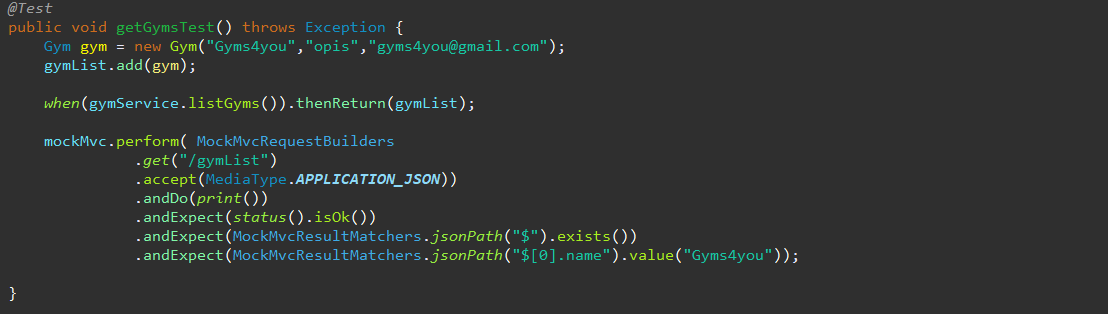
\includegraphics[scale=0.5]{slike/getGyms.PNG} %veličina slike u odnosu na originalnu datoteku i pozicija slike
    			\centering
    			\label{fig:promjene}
    	    \end{figure}
	

			\noindent \underbar{\textbf{2. Dodaj novu teretanu}}
			
            Ovdje smo testirali pokušaj dodavanja nove teretane odlaskom na /addGym  dok smo ulogirani kao role owner.

			\begin{figure}[H]
    			\hspace*{-1.5cm}
    			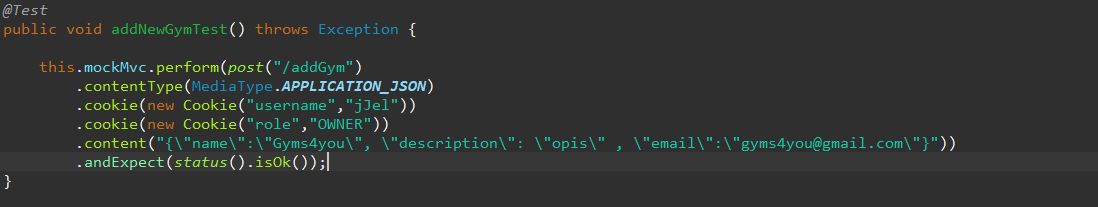
\includegraphics[scale=0.5]{slike/addNewGym.PNG} %veličina slike u odnosu na originalnu datoteku i pozicija slike
    			\centering
    			\label{fig:promjene}
    	    \end{figure}
	

			\noindent \underbar{\textbf{3. Dohvati trenerovu teretanu}}
			
			Ovdje smo testirali pokušaj dohvaćanja teretane u kojoj radi određeni trener odlaskom na /myGyms sa trenutnim ulogiranim trenerom.

			\begin{figure}[H]
    			\hspace*{-1.5cm}
    			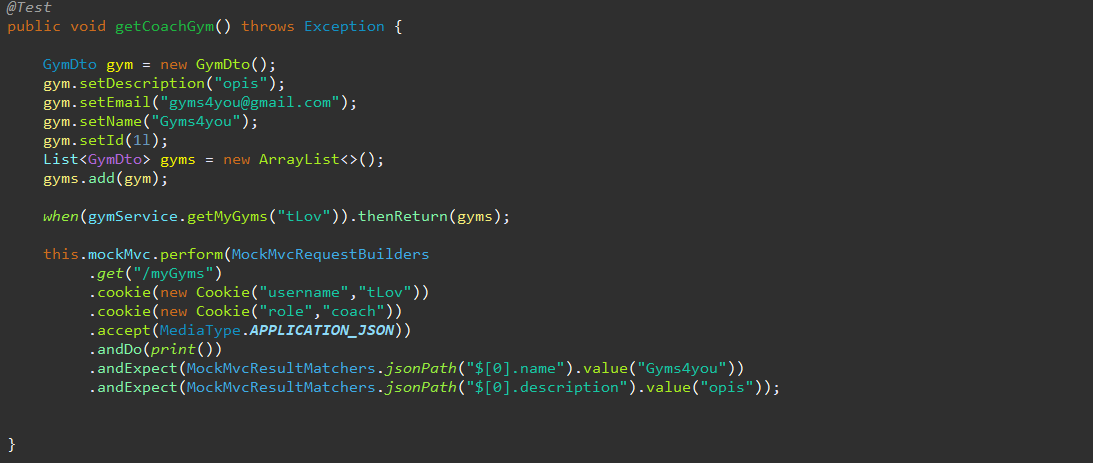
\includegraphics[scale=0.5]{slike/getCoachGym.PNG} %veličina slike u odnosu na originalnu datoteku i pozicija slike
    			\centering
    			\label{fig:promjene}
    	    \end{figure}
	
				
			\noindent \underbar{\textbf{4. Dohvati informacije o teretani}}
			
			Ovdje smo testirali pokušaj dohvaćanja informacija o određeneoj teretani odlaskom na /gymInfo sa pripadnim parametrom id koji se šalje preko URL-a.
             
			\begin{figure}[H]
    			\hspace*{-1.5cm}
    			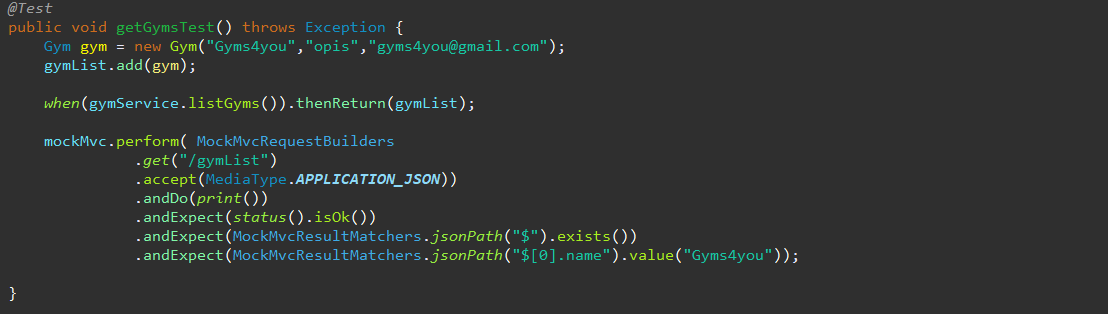
\includegraphics[scale=0.5]{slike/getGyms.PNG} %veličina slike u odnosu na originalnu datoteku i pozicija slike
    			\centering
    			\label{fig:promjene}
    	    \end{figure}
	

			\noindent \underbar{\textbf{5. Pronađi trenera}}
			
			Ovdje smo testirali pokušaj dohvaćanja trenera odlaskom na /coach sa pripadnim parametrom username koji se šalje preko URL-a.

			\begin{figure}[H]
    			\hspace*{-1.5cm}
    			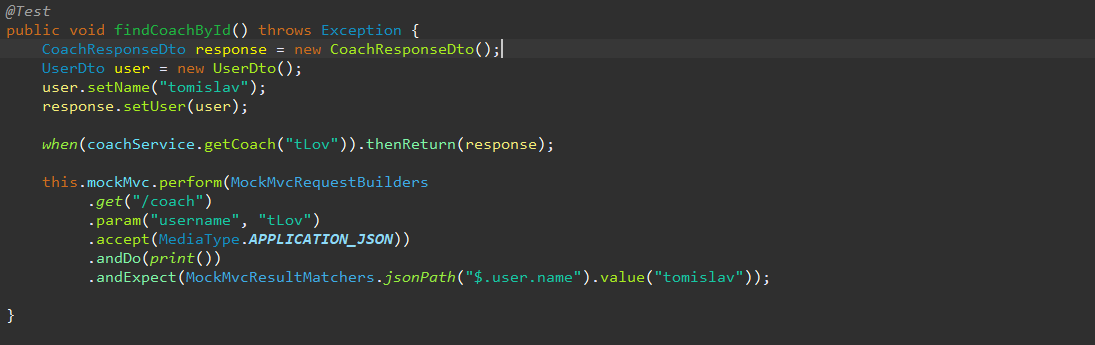
\includegraphics[scale=0.5]{slike/findCoachBy.PNG} %veličina slike u odnosu na originalnu datoteku i pozicija slike
    			\centering
    			\label{fig:promjene}
    	    \end{figure}
	

				
			\noindent \underbar{\textbf{6. Pronađi trenera (error) }}
			
			 Ovdje smo testirali pokušaj dohvaćanja trenera odlaskom na /coach bez parametra username kako bi dobili response 4xx koji javlja da je došlo do pogreške.
			\begin{figure}[H]
    			\hspace*{-1.5cm}
    			
\includegraphics[scale=0.5]{slike/findCoachByError.PNG} %veličina slike u odnosu na originalnu datoteku i pozicija slike
    			\centering
    			\label{fig:promjene}
    	    \end{figure}
	

				
			\noindent \underbar{\textbf{Prikaz prolaza svih ispita}}

			\begin{figure}[H]
    			\hspace*{-1.5cm}
    			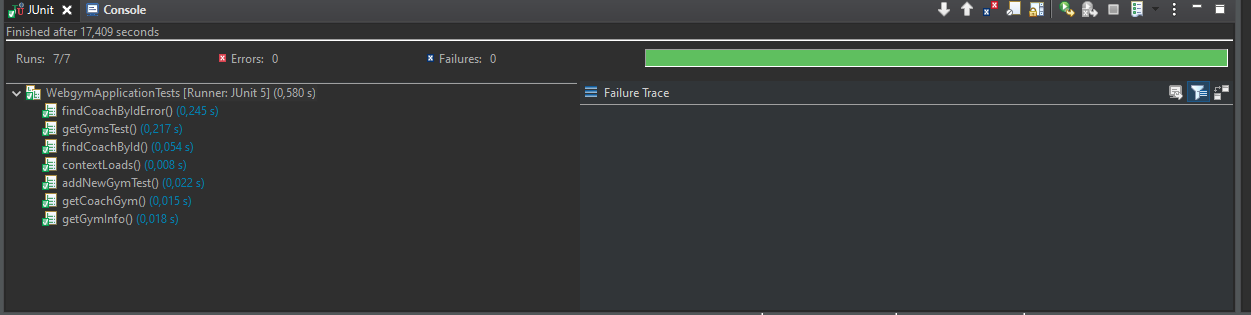
\includegraphics[scale=0.5]{slike/rezultati.PNG} %veličina slike u odnosu na originalnu datoteku i pozicija slike
    			\centering
    			\label{fig:promjene}
    	    \end{figure}
	

			\subsection{Ispitivanje sustava}
		
		 	 Za ispitivanje funkcionalnosti sustava koristili smo Selenium IDE. Testirali smo
		 	 sve obrazce uporabe te smo prolazili kroz aplikaciju i gledali općenito ponašanje
		 	 u nadi da pronađemo neko neočekivano hazardno ponašanje u svrhu otklonuća problema.
		 	 Neke od testiranih obrazaca uporabe smo prikazali u nastavku. ( UC1, UC2, UC3, UC7).
		 	 
		 	 
	
	            \noindent \underbar{\textbf{1. Ispitni slučaj (UC1 : Pregled teretana)}}
                \begin{packed_item}
						\item  \textbf{Ulaz : } 
						\item[] \begin{packed_enum}
	
							\item korisnik je pritisnuo na "popis teretana"

						\end{packed_enum}
						\item  \textbf{Očekivani rezultat: } 
						\item[] \begin{packed_enum}
	
							\item korisnik je dobio prikaz svih teretana

						\end{packed_enum}
						
						\item  \textbf{rezultat : }
						\item[] \begin{packed_enum}
	
							\item rezultat je jednak očekivanom rezultatu.

						\end{packed_enum}

				\end{packed_item}
				
				\begin{figure}[H]
        			\hspace*{-1.5cm}
        			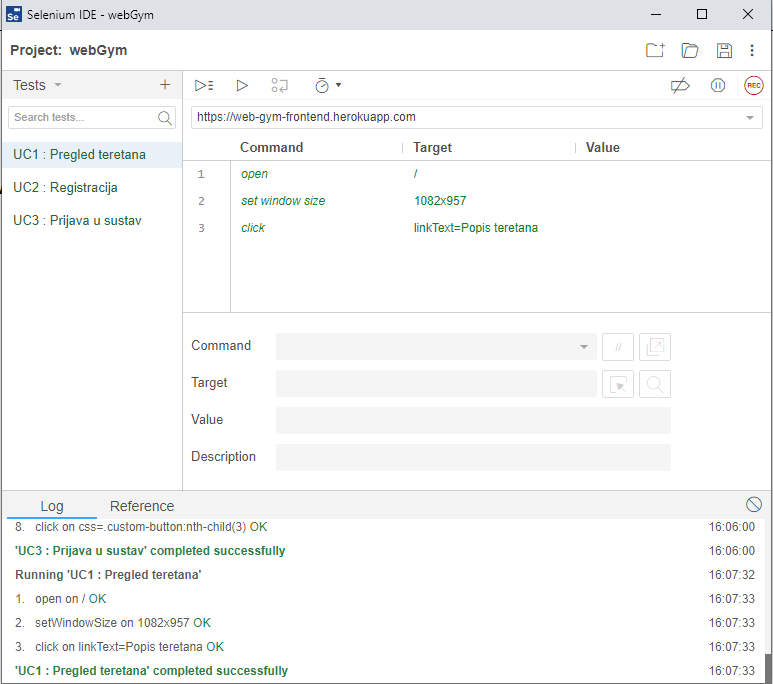
\includegraphics[scale=0.5]{dijagrami/UC1.PNG} %veličina slike u odnosu na originalnu datoteku i pozicija slike
        			\centering
        			\label{fig:promjene}
	        	\end{figure}
				
				\noindent \underbar{\textbf{2. Ispitni slučaj (UC2 : Registracija korisnika)}}
                \begin{packed_item}
						\item  \textbf{Ulaz : } 
						\item[] \begin{packed_enum}
	
							\item korisnik je pritisnuo na "prijava"
							\item korisnik je ispunio obrazac "registracija"
							\item korisnik je pritisnuo "registriraj"

						\end{packed_enum}
						\item  \textbf{Očekivani rezultat: } 
						\item[] \begin{packed_enum}
	
							\item korisnik se uspješno registrirao i spremio u bazu podataka

						\end{packed_enum}
						
						\item  \textbf{rezultat : }
						\item[] \begin{packed_enum}
	
							\item rezultat je jednak očekivanom rezultatu.

						\end{packed_enum}

				\end{packed_item}
				
				\begin{figure}[H]
        			\hspace*{-1.5cm}
        			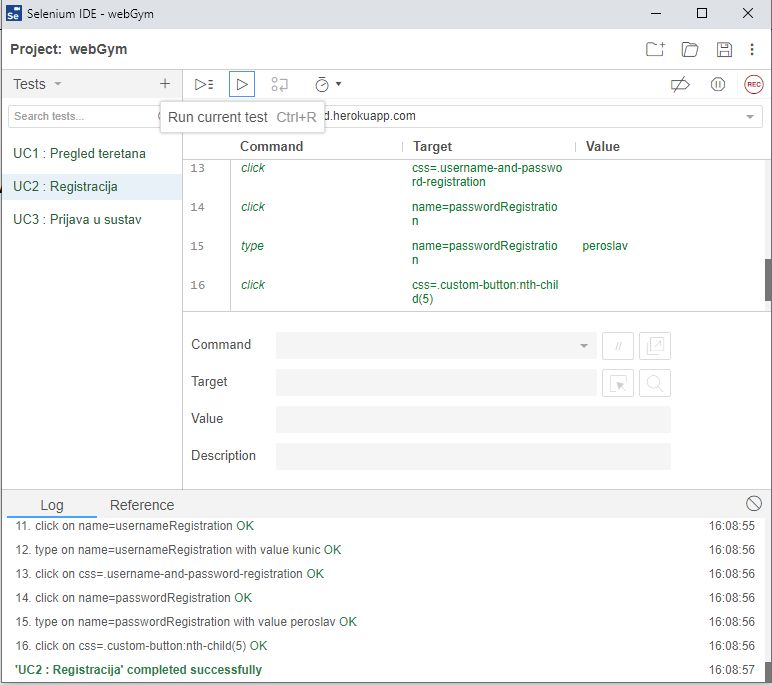
\includegraphics[scale=0.5]{dijagrami/UC2.PNG} %veličina slike u odnosu na originalnu datoteku i pozicija slike
        			\centering
        			\label{fig:promjene}
	        	\end{figure}
				
				\noindent \underbar{\textbf{3. Ispitni slučaj (UC3 : Prijava u sustav)}}
                \begin{packed_item}
						\item  \textbf{Ulaz : } 
						\item[] \begin{packed_enum}
	
							\item korisnik je pritisnuo na "prijava"
							\item korisnik je ispunio obrazac "prijava"
							\item korisnik je pritisnuo "prijava"

						\end{packed_enum}
						\item  \textbf{Očekivani rezultat: } 
						\item[] \begin{packed_enum}
	
							\item korisnik se uspješno prijavio u sustav

						\end{packed_enum}
						
						\item  \textbf{rezultat : }
						\item[] \begin{packed_enum}
	
							\item rezultat je jednak očekivanom rezultatu.

						\end{packed_enum}

				\end{packed_item}
				
				\begin{figure}[H]
        			\hspace*{-1.5cm}
        			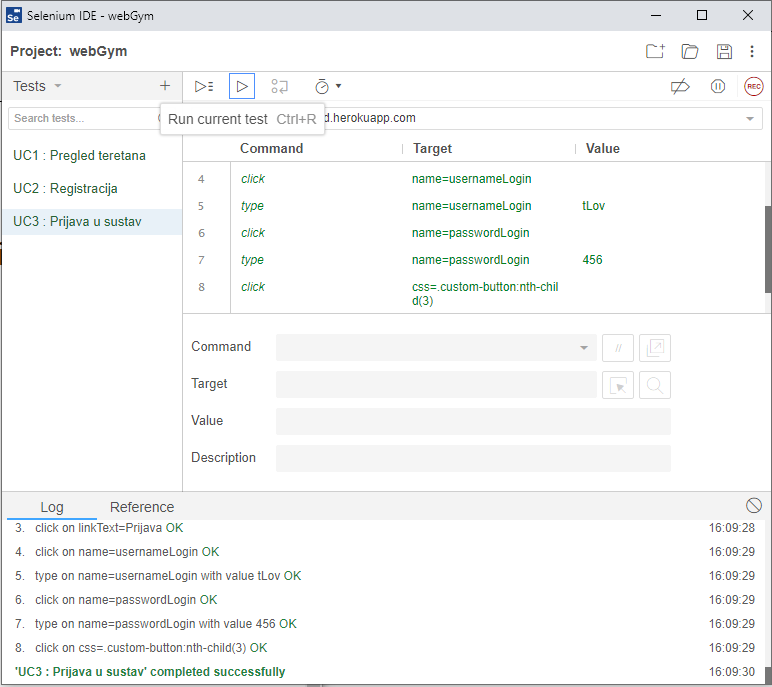
\includegraphics[scale=0.5]{dijagrami/UC3.PNG} %veličina slike u odnosu na originalnu datoteku i pozicija slike
        			\centering
        			\label{fig:promjene}
	        	\end{figure}
				
				\noindent \underbar{\textbf{4. Ispitni slučaj (UC7 : Pregled specifične teretane)}}
                \begin{packed_item}
						\item  \textbf{Ulaz : } 
						\item[] \begin{packed_enum}
	
							\item korisnik je pritisnuo na "Popis teretana"
							
							\item korisnik je pritisnuo na gumb informacije

						\end{packed_enum}
						\item  \textbf{Očekivani rezultat: } 
						\item[] \begin{packed_enum}
	
							\item korisnik je dobio informacije o odabranoj teretani

						\end{packed_enum}
						
						\item  \textbf{rezultat : }
						\item[] \begin{packed_enum}
	
							\item rezultat je jednak očekivanom rezultatu.

						\end{packed_enum}

				\end{packed_item}
					\begin{figure}[H]
        			\hspace*{-1.5cm}
        			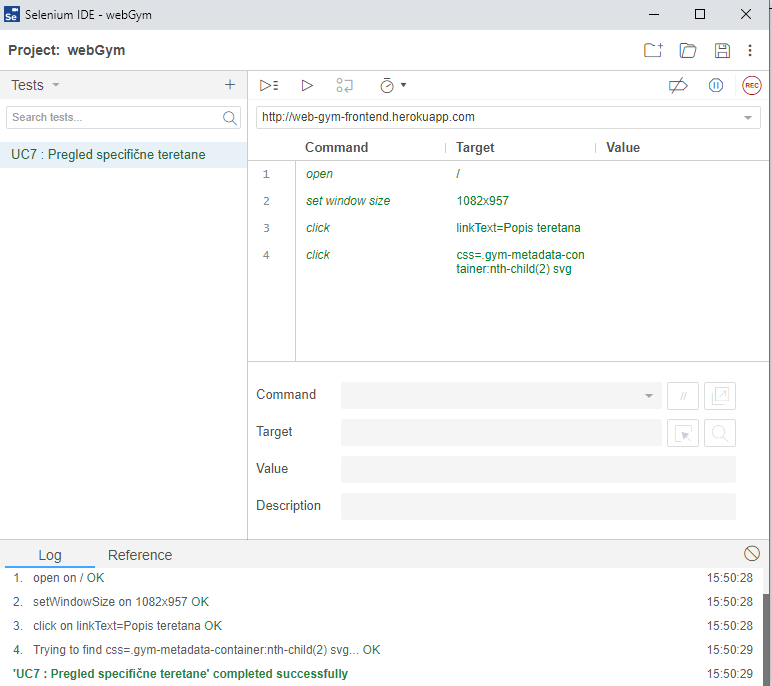
\includegraphics[scale=0.5]{slike/teretana.PNG} %veličina slike u odnosu na originalnu datoteku i pozicija slike
        			\centering
        			\label{fig:promjene}
	        	\end{figure}
	        	
	        \noindent \underbar{\textbf{5. Ispitni slučaj (UC20 : Pregled trenerove ponude)}}
                \begin{packed_item}
						\item  \textbf{Ulaz : } 
						\item[] \begin{packed_enum}
	
							\item trener je pritisnuo na "Moji planovi"

						\end{packed_enum}
						\item  \textbf{Očekivani rezultat: } 
						\item[] \begin{packed_enum}
	
							\item trener je dobio prikaz svih svojih planova treninga

						\end{packed_enum}
						
						\item  \textbf{rezultat : }
						\item[] \begin{packed_enum}
	
							\item došlo je do pogreške te se nisu učitali trenerovi planovi.
                                                
                            - Do pogreške je došlo zbog problema u pamćenju cookie-a koje smo naknadno riješili, a problem je bio u tome što su se uloge korisnika pamtile na krivi način te korisnik od strane sustava nije bio prepoznat kao trener.
                        
						\end{packed_enum}

				\end{packed_item}
					\begin{figure}[H]
        			\hspace*{-1.5cm}
        			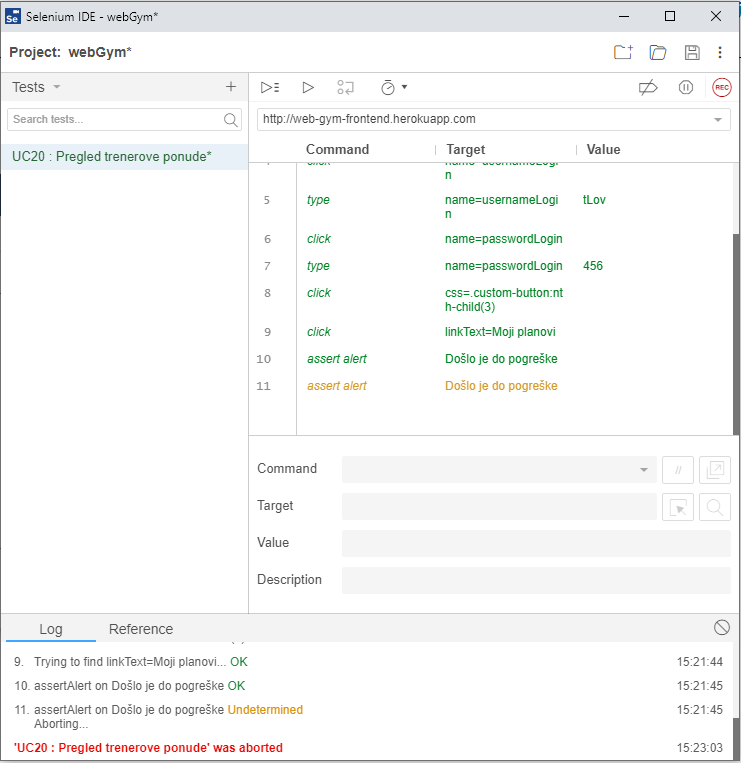
\includegraphics[scale=0.5]{slike/error.PNG} %veličina slike u odnosu na originalnu datoteku i pozicija slike
        			\centering
        			\label{fig:promjene}
	        	\end{figure}
		 
			\eject 
			
			
		\section{Dijagram razmještaja}
		
		Dijagram razmještaja prikazuje generalnu topologiju sustava koji se koristi kako bi resursi bili optimalno raspoređeni. Predstavlja statički pogled na razmještaj sklopovskih i programskih komponenata. Na poslužiteljskom računalu se nalaze web poslužitelj, poslužitelj baze podataka i poslužitelj za frontend. Klijenti koriste web preglednik kako bi pristupili web aplikaciji. U bazi podataka sadržane su sve potrebne informacije i datoteke koje korisnik može zahtijevati. Sustav je baziran na arhitekturi ”klijent – poslužitelj”. Komunikacija između poslužiteljskog računala i klijentskog računala se omogućuje HTTP protokolom. 
		
		
		
		\begin{figure}[h]
			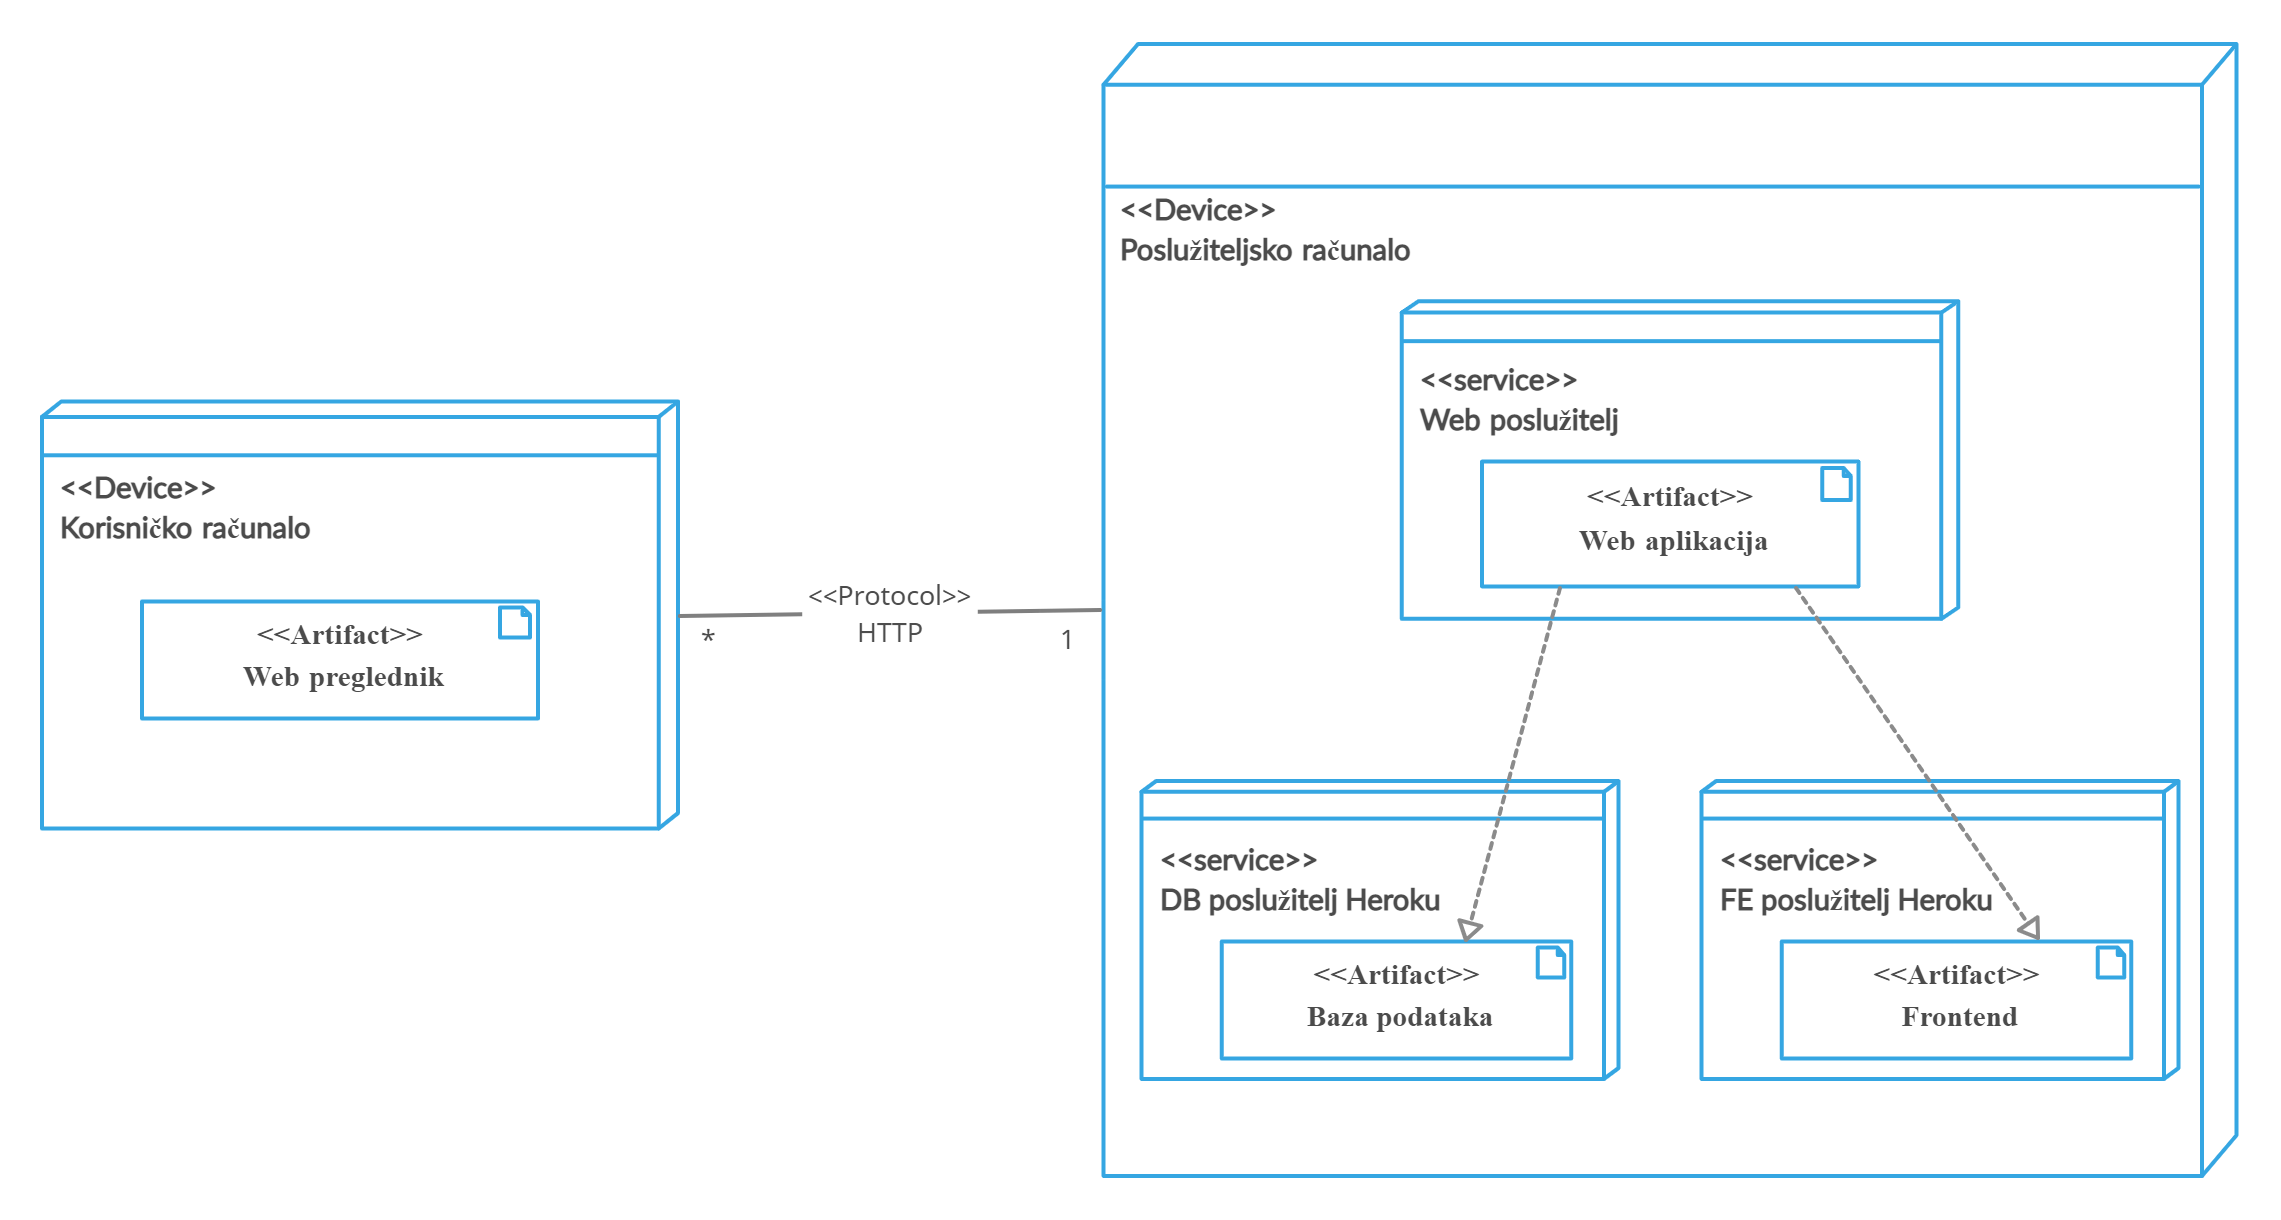
\includegraphics[height=                       9cm,width=1\textwidth]{dijagrami/Dijagram_razmjestaja.png}
			\begin{center}
				Slika 5.1: Dijagram razmještaja
			\end{center}
		\end{figure}
		
		\eject	
		
		
		\section{Upute za puštanje u pogon}

		    \begin{packed_item}
						\item  \textbf{1. Stvaranje backend heroku servera} 
						\item[] \begin{packed_enum}
	
							\item Stvaranje account-a na https://dashboard.heroku.com/
							
							\item Instalacija Heroku CLI : https://devcenter.heroku.com/articles/heroku-cli
							
							\item Otvaranje command prompt-a
							
							\item Unos "heroku create "NAME-OF-APP" (webGym) ili samo "heroku create"
							
							    - U slučaju da se ne navede ime aplikacije , i dalje će se stvoriti server ali s random imenom koji je kasnije moguće preimenovati u željeno ime.
							
							\item Stvoren je server.
							    
							    \begin{figure}[H]
                        			\hspace*{-1.5cm}
                        			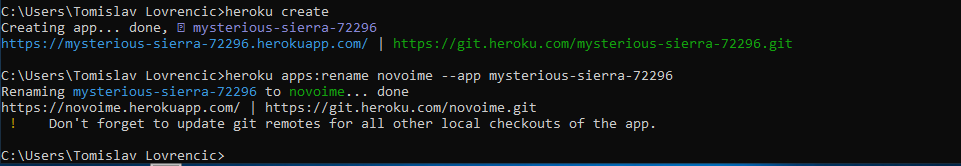
\includegraphics[scale=0.5]{dijagrami/cmd.PNG} %veličina slike u odnosu na originalnu datoteku i pozicija slike
                        			\centering
                        			\label{fig:promjene}
                        		\end{figure}

						\end{packed_enum}
						\item  \textbf{2. Konfiguracija baze podataka} 
						\item[] \begin{packed_enum}
	
							\item Odlazak na stranicu  https://dashboard.heroku.com/
							
							\item Klik na stvoreni server. (novoime)
							
							\item Klik na resources
							
							\item Pronaći pod add-ons  Heroku POSTGRES
							
							    - Odabrati Hobby dev - FREE
							  
							
							\item Stisnuti na SUBMIT FORM.
							
							\item Stvorena je baza podataka
							    
							    \begin{figure}[H]
                        			\hspace*{-1.5cm}
                        			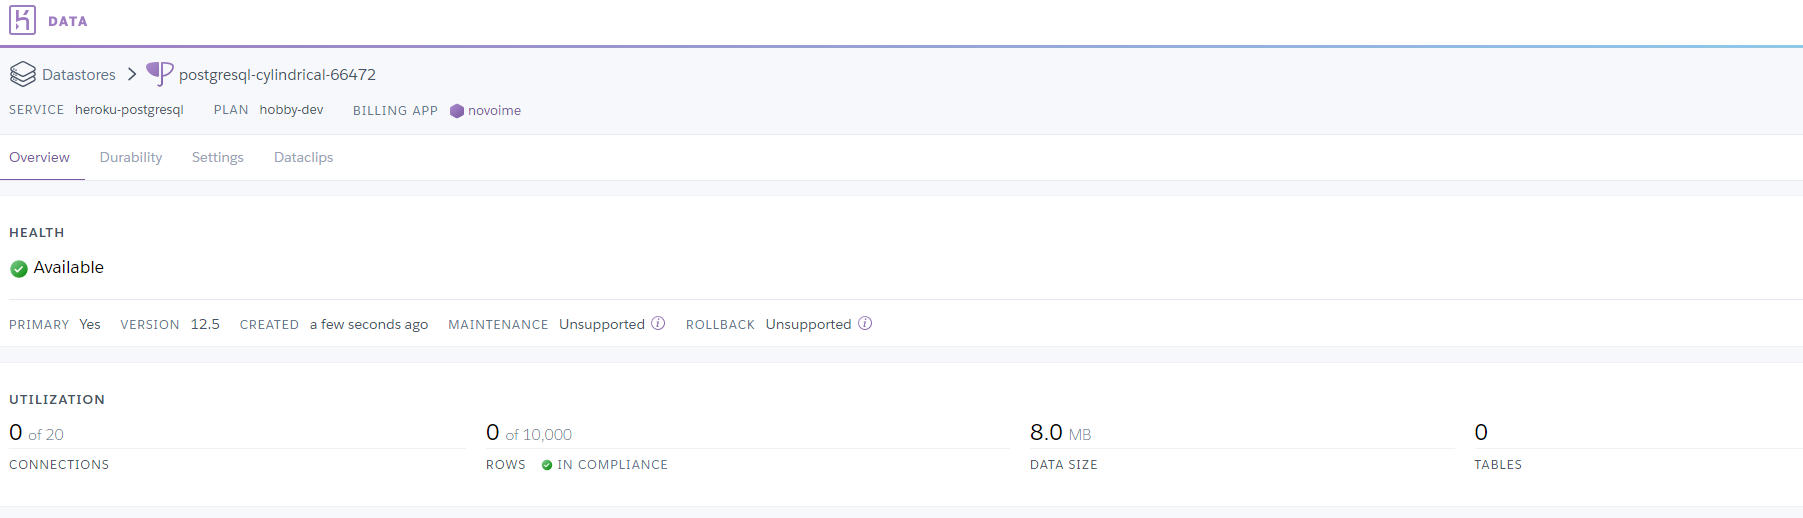
\includegraphics[scale=0.3]{dijagrami/baza.PNG} %veličina slike u odnosu na originalnu datoteku i pozicija slike
                        			\centering
                        			\label{fig:promjene}
                        		\end{figure}

						\end{packed_enum}
						
						
						\item  \textbf{3. Spajanje backend servera na stvorenu bazu u Heroku}
						\item[] \begin{packed_enum}
	
							\item Odlazak na stranicu  https://dashboard.heroku.com/
							
							\item Klik na stvoreni server: "novoime" (za potrebu ovih uputa koristit ćemo "novoime" kao ime)
							
							\item Klik na resources
							
							\item Klik na Heroku POSTGRES
							
							\item Klik na settings
							
							\item Klik na view credentials
							
							\item Otvoriti backend kod (Java)
							
							\item Odlazak u src/main/resources/application.properties
							
							\item Konfiguracija :
							    
							       - Potrebno je podesiti backend tako da se povezuje sa bazom koju smo u prethodnom koraku stvorili na Heroku.
							       
							       - U tom naumu ćemo morati podesiti spring.datasource.url , spring.datasource.username te spring.datasource.password na način da ćemo pročitati vrijednosti koje nam je dao Heroku credentials i nadodati ih na spomenute vrijednosti.
							       
							       - Zadnja napomena je dodavanje "jdbc:" na početak URI-a koje nam je generirao heroku.
						
							    \begin{figure}[H]
                        			\hspace*{-1.5cm}
                        			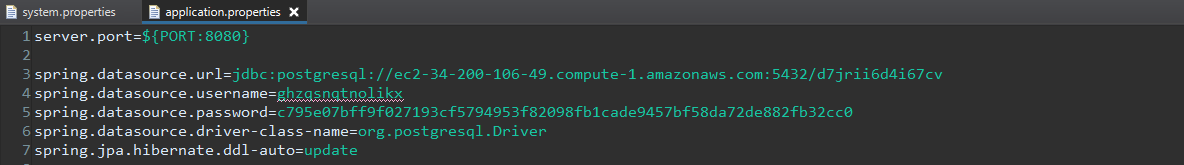
\includegraphics[scale=0.5]{slike/java.PNG} %veličina slike u odnosu na originalnu datoteku i pozicija slike
                        			\centering
                        			\label{fig:promjene}
                        		\end{figure}

						\end{packed_enum}
						
						\item  \textbf{4. deploy backend-a}
						\item[] \begin{packed_enum}
	
							\item Otvoriti backend project.
							
							\item Otvoriti pom.xml te dodati potrebni plugin:
			
							    \begin{figure}[H]
                        			\hspace*{-1.5cm}
                        			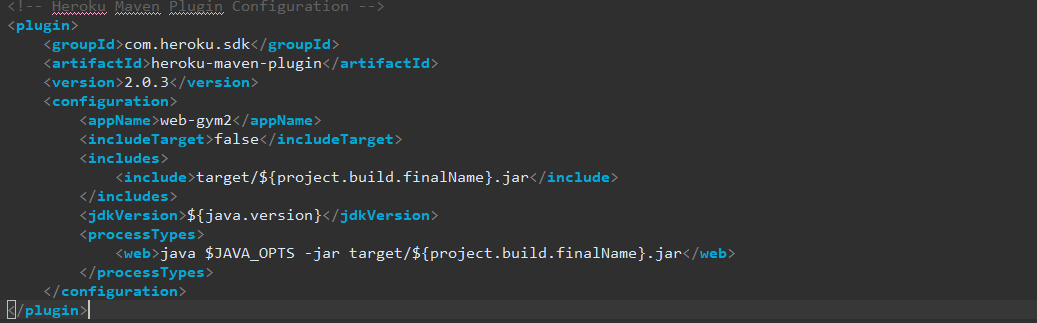
\includegraphics[scale=0.5]{slike/plugin.PNG} %veličina slike u odnosu na originalnu datoteku i pozicija slike
                        			\centering
                        			\label{fig:promjene}
                        		\end{figure}
                        		
                        		- Napomena : prateći ranije opisane korake za appName trebali bi napisati
                        		"novoime", a u našem slučaju to je "web-gym2".
							
							\item Otvoriti cmd te se pozicionirati u root backend projekta
							
							\item Napisati "mvn clean heroku:deploy"
						

						\end{packed_enum}
						
				\item  \textbf{5. Stvaranje frontend servera te deploy frontend-a}
				\item[] \begin{packed_enum}
	
							\item Odlazak na stranicu  https://dashboard.heroku.com/
							
							\item Otvoriti cmd te upisati "heroku create NAME-OF-FRONTEND-APP --buildpack https://github.com/mars/create-react-app-buildpack.git"

							\item Napraviti prazan folder , unutar foldera u cmd-u napisati "git init"
							
							\item U cmd-u napisati "heroku git:remote -a NAME-OF-FRONTEND-APP"
							
							\item Prekopirati root frontend projekta u stvoreni folder
							
							\item Dodati static.json datoteku u root frontend projekta
							    
							    \begin{figure}[H]
                        			\hspace*{-1.5cm}
                        			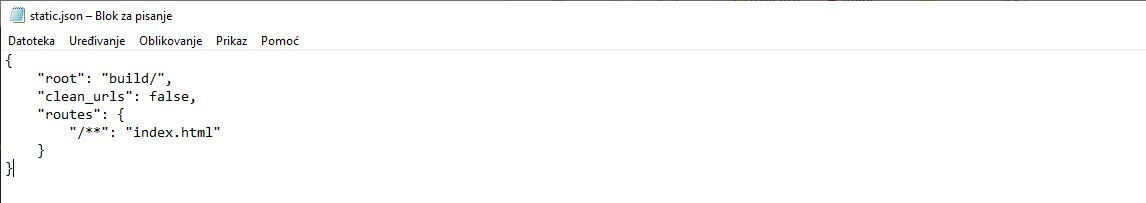
\includegraphics[scale=0.5]{slike/json.PNG} %veličina slike u odnosu na originalnu datoteku i pozicija slike
                        			\centering
                        			\label{fig:promjene}
                        		\end{figure}
							
							\item prije deploya frontenda , ući u src/App.js te promjeniti backend URL i 
							postaviti ga na URL servera backenda.
							
							    \begin{figure}[H]
                        			\hspace*{-1.5cm}
                        			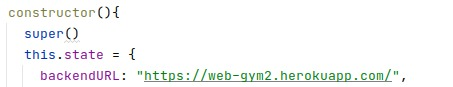
\includegraphics[scale=0.7]{slike/front.png} %veličina slike u odnosu na originalnu datoteku i pozicija slike
                        			\centering
                        			\label{fig:promjene}
                        		\end{figure}
							
							\item U cmd upisati "git add ."
							
							\item U cmd upisati "git add -m "initial commit""
							
							\item U cmd upisati "git push heroku master"
	

						\end{packed_enum}

				\end{packed_item}
				
			\eject 